\renewcommand{\prechaptername}{付録}
\renewcommand{\postchaptername}{}
\renewcommand{\thechapter}{\Alph{chapter}}

\chapter{光の量子状態について}


\begin{figure}[htbp]
        \centering   
        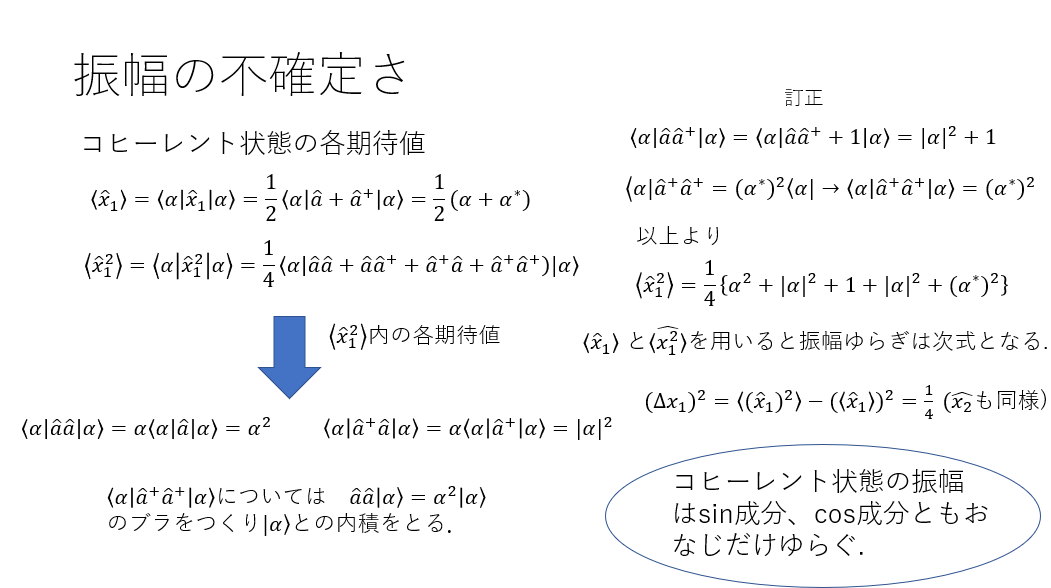
\includegraphics[width=0.8\textwidth]{img/zemi20.png}
        \caption[sample image (png)]{振幅の不確定さ.}
        \label{Fig:1_7_5}
    \end{figure}
    
\begin{figure}[htbp]
        \centering   
        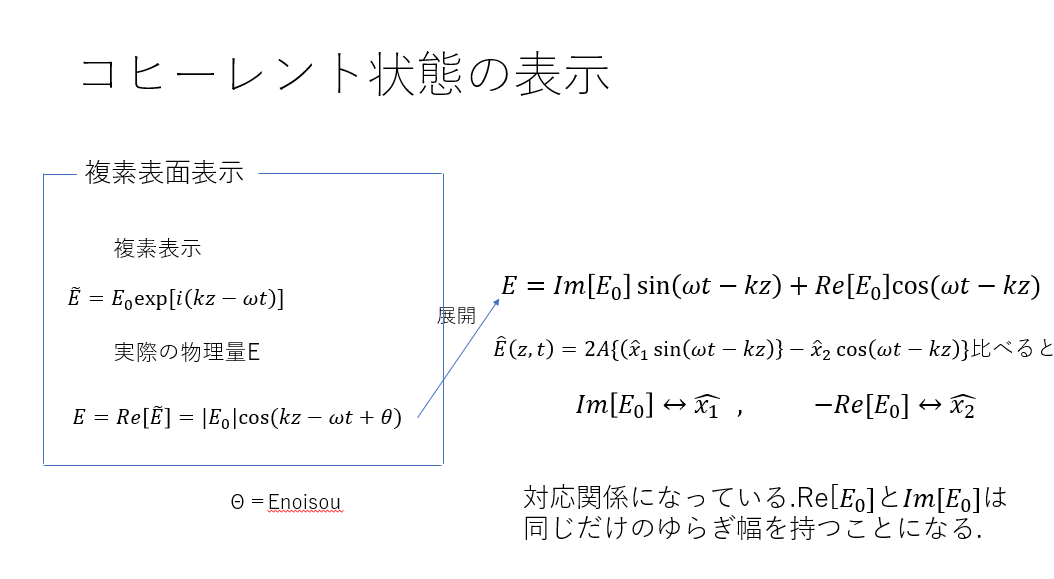
\includegraphics[width=0.8\textwidth]{img/zemi21.png}
        \caption[sample image (png)]{コヒーレント状態の表示.}
        \label{Fig:1_7_6}
    \end{figure}
    
\begin{figure}[htbp]
        \centering   
        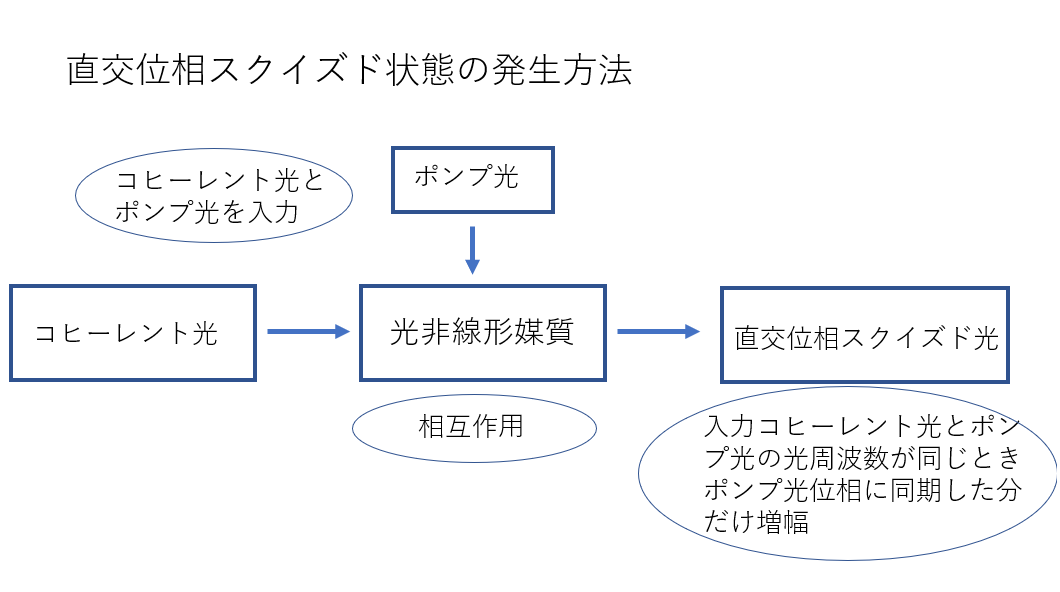
\includegraphics[width=0.8\textwidth]{img/zemi22.png}
        \caption[sample image (png)]{直交位相スクイズド状態の発生方法.}
        \label{Fig:1_7_7}
    \end{figure}